\documentclass[12pt,a4paper]{article}
\usepackage[utf8]{inputenc}
\usepackage[spanish]{babel}
\usepackage{amsmath}
\usepackage{amsfonts}
\usepackage{amssymb}
\usepackage{makeidx}
\usepackage{graphicx}
\usepackage{lmodern}
\usepackage{kpfonts}
\usepackage{fourier}
\usepackage[left=2cm,right=2cm,top=2cm,bottom=2cm]{geometry}
\author{Rodriguez Lopez Francisco Javier}
\begin{document}

\begin{center}
\LARGE \textbf{Universidad Politecnica de la Zona Metropoilitana de Guadalajara\\}



\includegraphics[scale=1]{Upzmg5.png} 

\large \textbf{Diseño del Puente H}\\
\vspace{1cm}
\large \textbf{Nombre:\\
Guzmán Vazquez Jaime Alan Yamil.\\
Ródriguez López Francisco Javier.\\
\vspace{0.5cm} Matrícula:\\
18311861\\
18311804.\\
\vspace{0.5cm} Carrera: Ingeniería en Mecatrónica.\\
\vspace{0.5cm} Materia: Sistemas Electrónicos de Interfaz.\\
\vspace{0.5cm} Curso: septiembre-noviembre del 2019.\\
\vspace{0.5cm} Docente: Morán Garabito Carlos Enrique.}


\vspace{4cm}
\small \textbf{31 de Octubre del 2019}
\end{center}


\section{Introducción:}
En este documento se explicara todo lo referente a la practica que se realizo con anterioridad, el puente H que se realizo mediante mosfet y el control de la placa ARDUINO UNO  para controlar el cambio de los reveladores del mismo puente, estos detalles serán abordados a detalle en este documento ademas de explicar la programación que se utilizo en el ARDUINO  para que  realizara su función de controlador.\\

Se explicara ademas el funcionamiento de cada parte del circuito teniendo en cuenta su funcionamiento y porque se realizo así, se explicara el porque del motor utilizado y su funcionamiento en conjunto con el puente H,
Al igual que se abordaran los temas descritos anteriormente como lo son la programación y el armado se  explicaran apartados como los cálculos necesarios para dicha practica, ya  sea calculo que se necesito para las resistencias y determinar su valor para evitar que ya sea el arduino, los reveladores o incluso el motor o los mosfets resultaran quemados, esto se explicara a fondo al igual que los aspectos anteriores en el apartado de procedimiento.\\
  
Se mostraran los resultados de la practica realizada en el apartado resultados en donde se mostrara los circuitos utilizados para esta labor, Ademas de mostrar el diagrama que se utilizo para ademas de enumerar las modificaciones que se realizaron al diagrama que se nos fue entregado por defecto debido a que se le realizaron cambios puesto que el diagrama original utilizaba otro tipo de controlador.

\section{Objetivo:}
Realizar el cambio de polaridad de un motor eléctrico por medio de un puente H.

\section{Procedimiento:}

\subsection{Programacion:}

Para realizar la programación se tuvo que desarrollar un programa que en el momento que el usuario presionara un botón el ARDUINO mandara una señal de 5 voltios a el revelador, activandolo para esto se debe tomar en cuenta que el se debe estructurar la programación de forma en la que los pines de entrada sean de forma análogos, mientras que los pines de salida sean digitales para poder generar los 5 voltios que se desean en la placa arduino puesto que de ser programado entradas y salidas de manera digital el arduino solo registrara 3.3 voltios de salida por cuestiones de diseño del mismo.\\
Esta misma función se realizara dos veces, es decir programar dos entradas y dos salidas, una para cada botón que cada una saldrán a cada revelador, cada una activaran la polarización ya sea hacia una direccion del motor o ya sea hacia la otra generando la función requerida para el puente H.\\

Comenzemos por declarar las variables de entrada y de salida para el circuito, esto se realiza antes de el apartado\\ VOID LOOP  y antes de VOID SETUP.
Para declarar variables basta con poner la variable junto con el pin de salida que tendrá es decir:\\
SALIDA=13;\\
ENTRADA=A0;\\

En este apartado dices que la variable SALIDA sera dirigida a el pin numero 13 del arduino que es un pin digital y la variable ENTRADA sera dirigida al pin numero A0 del arduino que es un pin analogo.\\\\
Después de declara los pines correspondientes se procederá a declara esos pines como entrada o como salida debido a que en el apartado anterior solamente los declaraste para que se tomaran en cuenta mas no para que sirvieran como receptores o  emisores de energía.\\\\
Esto se realiza en el apartado VOID SETUP en donde se declaran los pines de manera en que sirvan como salida o entrada de la siguiente forma:\\\\

VOID SETUP(){\\
PinMode(SALIDA,OUTPUT);\\
PinMode (ENTRADA,INPUT);\\

En esta parte seleccionas la variable SALIDA como sal
]else[digitalWrite(SALIDA,LOW)]\\

En esta sección se programa que en caso de que la variable ENTRADA este recibiendo voltaje entonces la variable  SALIDA enviara los 5 voltios de los que se trato anteriormente teniendo la activación del revelador para la función consiguiente del puente H.\\
Este proceso se realiza dos veces es decir como nosotros necesitamos dos salidas y dos entradas estas el proceso solo se repetirá dos veces agregando dos variables mas y realizando el mismo proceso de nuevo. Dando salida como una variable y la variable ENTRADA como entrada.\\\\

Después de declara cada una de las variables como corresponde se procederá a realizar el proceso en el apartado VOID LOOP que sera lo que se repetirá durante todo el tiempo de funcionamiento del arduino.\\
VOID LOOP()\\
if(AnalogRead(ENTRADA,HIGH))\\

[DigitalWrite(SALIDA,HIGH)\\

\subsection{Conexiones:}

Entre las conexiones, para la obtencion del puente H, se tienen las mismas interfaces tanto de entrada que esta complementada por optoacopladores, y la de salida acoplada a los relevadores y diodos. Teniendo en cuenta lo que se ha estado trabajando en las anteriores practicas, la unica conexion nueva es la del puente H.\\

Entre la conexion del puente H, se tiene un diagrama, en donde involucra a los componentes MOSFET, estos componentes son lo mas relevante de esta practica, ya que en su interior tiene un diodo zener, y como un llamado a transistor, ya que tiene entradas, emisor y conector, esta vez llamada, source, gate y deam, este componente trae eso en su interior, y nos ayuda a la hora de ver la polaridad del motor, ya que este puede ser controlado a partir de tener en acoplamiento, un diodo y un transmitor de señales. El diagrama establecido para esta practica es el siguiente:\\

\begin{center}
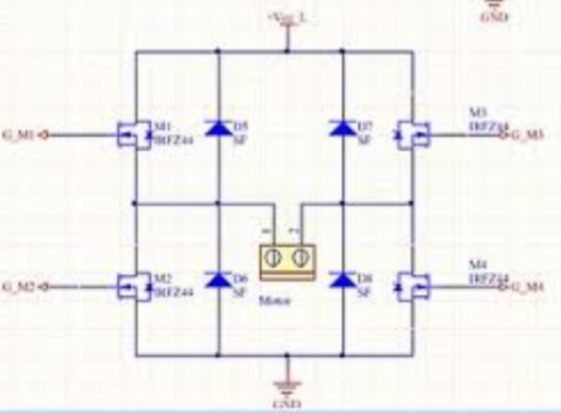
\includegraphics[width=10cm]{Diagrama.png} 
\end{center}

Como se puede apreciar en el diagrama, los mosfet estan conectados entre si, dejando los cuatro componentes que se ven, dos en serie, y entre ellos dos en parelelo, esto para intervenir a la hora de conexion entre cada MOSFET, en donde se puede apreciar como entre el MOSFET que esta en diagonal al otro MOSFET, se conectan, esto para que el motor gire en un sentido, y entre ello la otra parte que es igual, en donde los MOSFET, estan conectados en diagonal, nuevamente.\\

Teniendo en cuenta las conexiones, y el rol que deben de cumplir, se debe de tener en cuenta, que tenemos que tener una fuente extra, conectada a la zona de los mosfet, ya que el motor, con el que se trabajara, dadas las interfaces que se tienen, y al arduino conectado, no es suficiente para alimentarlo, dadas las entradas de los MOSFETS, es por eso que se pone una fuente esto dado por el voltaje que se debe de tener, en este caso se utilizara una fuente de 8v, para que el giro del motor sea notable, dadas sus polaridades, y estas con sus entradas en las señales de salida \cite{munoz2016ensenando} .\\

En las conexiones dadas el diagrama, se ve que el source de uno va conectado al dream del que esta debajo de ello, entre los que estan en paralelo, se conecta en la parte de arriba dream con dream, y en la parte de abajo, es conectada source con source, y entre estas las gates de los primeros MOSFETS, en serie van las compuertas del relevador, en este caso, el normalmente abierto, para hacer correr la corriente que se necesita para el motor. y por ultimo el motor, que va conectado a un MOSFET en paralelo en la pata del dream, y lo mismo con el otro MOSFET, cuidando las polaridades, entre el motor y los dos MOSFETS, que estan en paralelo.

\section{Resultados:}

Teniendo en cuenta las conexiones y la programacion, en las que hay que guiarse, se lanzan resultados guiados en el puente H. En este punto se tiene por visto, que la funcion del puente H, es hacer girar un motor en sus dos polaridades.\\


Dadas las conexiones del los MOSFETS, este nos va a arrojar un voltaje dependiendo de con cuanto se este aliemntando, en este caso son 8 voltios, una vez sacado estos 8 voltios, el motor empezara a girar, esto cada que prsionemos el push botton, en las interfaces de entrada, activando el relevador, que se tiene conectado a ese push botton, y comunicandose asi con los mosfets, a los que se esten vinculando. Preciando que hay comunicacion entre las interfaces y los MOSFETS, esto gracias a un microprocesador en este caso, Arduino, que deja compatibilizar, las interfaces con el puente H, para hacer poder girar el motor en sus dos polaridades, cada una vinculada con un push botton,generando un voltaje en un boton, de forma positiva, y otro push botton en voltaje de forma negativa.\\

Dejando apreciar, que el voltaje cambia a negativo, dirigido, asi por la polaridad del motor en la que esta girando, ya sea este su polo comun, o el polo inversor, que en si es el objetivo de esta pratica.\\

\begin{center}
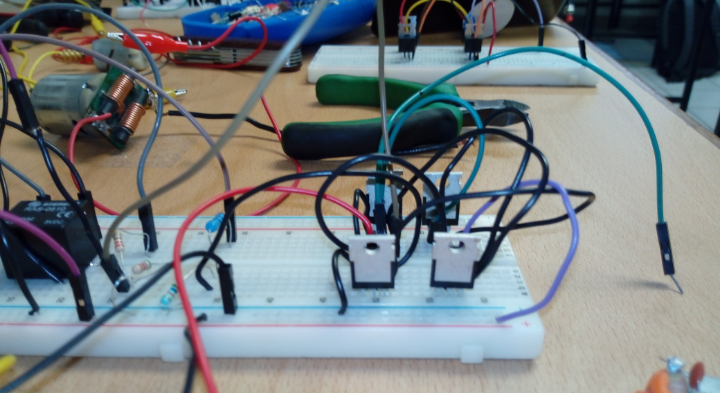
\includegraphics[width=10cm]{puenth.png} 
\end{center}

Esto como se ve en la imagen, son las conexiones que los MOSFETS, deben de tener para cumplir sus cambios de polaridad, se aprecia como entre estos se establece el voltaje al que va dirigido tanto los relevadores, como el motor, que va en su salida. Guiados por el diagrama, deben de estar las mismas conexiones que este.\\

Por ultimo, se ve la imagen, en donde se ven conectados las interfaces, con el microprocesador, y en su punto el puente H, en donde tenemos comunicacion una vez dada la sensates de tener bien las conexiones, presionando uno de los dos botones que se tienen, nos generara un voltaje de 5 voltios, que esto a su vez el relevador los recibira, y cuando lance su corriente y su voltaje, en el comun de este, se guiara al gate de este, lanzando una señal para la fuente independiente, generando que todo lo que se tenga en porcentual al motor, genere la corriente que se tiene establecida, para el rotor de este.\\

\begin{center}
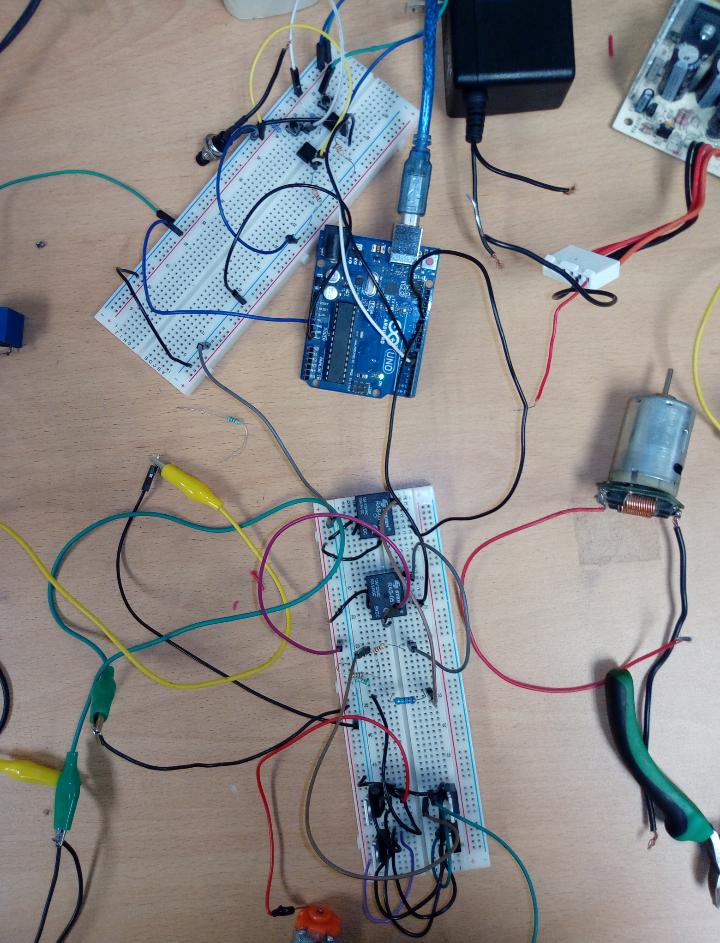
\includegraphics[width=6cm]{Circuito.png} 
\end{center}

\textbf{\LARGE Conclusión:}\\

\textbf{Jaime Alan Yamil Guzmán Vazquez.\\}
Esta practica tiene implicaciones muy importantes debido a que el uso del puente H es muy basto en el mundo de la electrónica y puede ser usado para muchas cosas puesto a esto es de gran importancia saber el funcionamiento de este ademas de que también se utilizan otros componentes como serian los mosfets y los reveladores que hacen su trabajo realizando el cambio de fase o de direccion del circuito, ademas de la importancia de la programación que se asemeja mucho a la programación como lo seria c estándar o incluso Phyton que cada vez nos da mas conocimientos y generan bases mucho mas grandes para la ingeniería que se cursa.\\

\textbf{Francisco Javier Ródriguez López:\\}
El puente H, es una herramienta muy utlizada desde ya hace tiempo, puesto que en ella podemos ver desde una vista mas basica, el giro de un motor, en sus dos polaridades, cada una de ellas funcionales en un torque, el cual ayuda a ver como podria trabajar la potencia entre las comunicaciones de esté, y sus relaciones entre otras razones más por las cuales, son necesarias tener en cuenta, si es que se quiere trabajar a futuro, con motores, como en el caso de brazos robóticos, o en cuestión de otros rangos a los que pueda ser utilizado, esto dada su necesidad que tiene, y con que frecuencia este se tiene en relevancia el giro de un motor, ya sea en un proyecto profesional, hasta cualquier herramienta en la cual se pueda adaptar.\\

Para asi pues, tener en cuenta con que trabajar, y como generar y trasmitir la potencia, corriente y voltaje que se esta relacionando al motor, y en caso como este componente (MOSFETS), dan un mejor control, y disparo a la hora de disipar la energia que circula por el circuito a analizar y trabajar.

\bibliographystyle{apalike}
\bibliography{ref}

\end{document}